\documentclass[11pt,a4paper]{article}
\usepackage[utf8]{inputenc}
\usepackage[T1]{fontenc}
\usepackage[margin=2cm]{geometry}
\usepackage{enumitem}
\usepackage{titlesec}
\usepackage{graphicx}
\usepackage{array}
\usepackage{tabularx}
\usepackage{xcolor}
\usepackage{hyperref}

% Use Times font
\usepackage{times}

% Define colors
\definecolor{darkblue}{RGB}{0,51,102}
\definecolor{gray}{RGB}{80,80,80}

% Section formatting
\titleformat{\section}{\Large\bfseries\color{darkblue}}{}{0em}{}[\titlerule]
\titlespacing*{\section}{0pt}{12pt}{6pt}

% Remove page numbering
\pagestyle{empty}

% Custom commands
\newcommand{\cvitem}[2]{\textbf{#1} & #2 \\[0.3em]}
\newcommand{\cventry}[4]{\textbf{#1} & #2 \\ & \textit{#3} \\ & #4 \\[0.5em]}

\begin{document}

% Header with photo and date
\begin{minipage}[t]{0.7\textwidth}
    \vspace{0pt}
    {\Huge\bfseries\color{darkblue} Michitoshi Tsubaki}
    \vspace{0.3cm}
    
    {\Large Undergraduate Student, JSK Robotics Lab.}\\
    Department of Mechano-Informatics\\
    Faculty of Engineering, The University of Tokyo
    \vspace{0.5cm}
    
    \textcolor{gray}{
    \textbf{Email:} tsubaki@jsk.t.u-toyko.ac.jp, michi.tsubaki.tech@gmail.com\\
    \textbf{Phone:} +81-90-6101-0564\\
    \textbf{LinkedIn:} linkedin.com/in/michi.tsubaki
    }
\end{minipage}
\hfill
\begin{minipage}[t]{0.25\textwidth}
    \vspace{0pt}
    \raggedleft
    \textcolor{gray}{\small \today}\\[0.3cm]
    \fbox{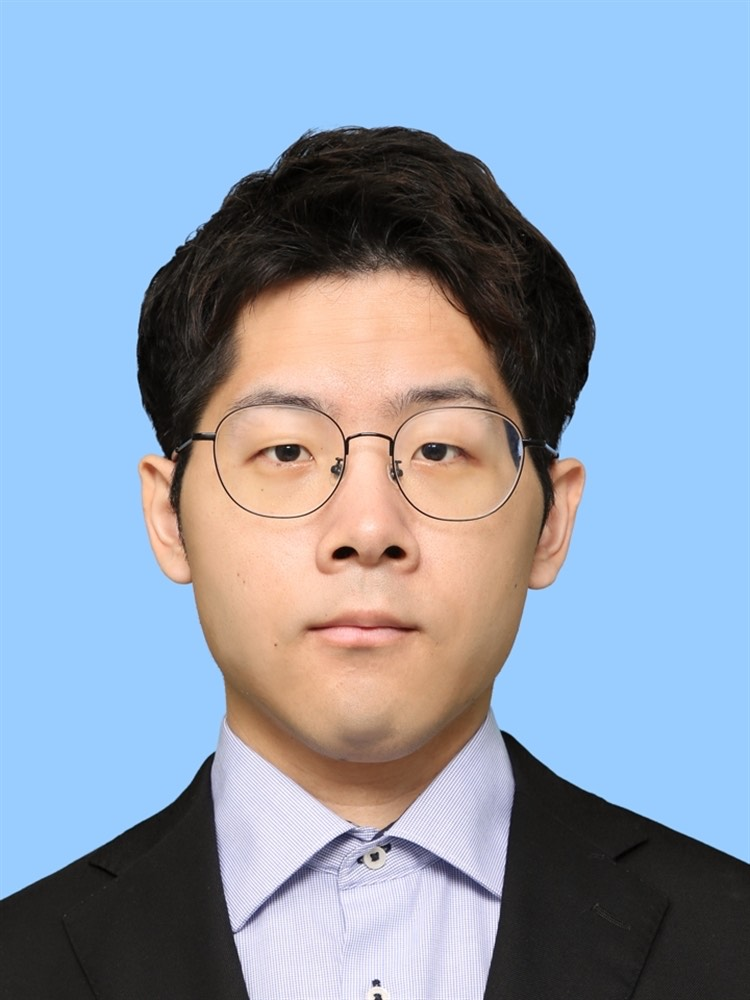
\includegraphics[width=\textwidth,height=3cm,keepaspectratio]{photo.jpeg}}
\end{minipage}

\vspace{1cm}

% Affiliations
\section{Affiliations}
\begin{itemize}[leftmargin=1cm,itemsep=0.2em]
    \item JSK Robotics Laboratory (PI : Prof. Dr. Kei Okada) : Undergraduate Student
    \item Proxima Technology Inc. : Part-time Engineer
\end{itemize}

% Education
\section{Education}
\begin{tabularx}{\textwidth}{@{}p{2.5cm}X@{}}
\cventry{2026(Scheduled)}{JSK Robotics Lab. (Supervised by Prof. Kei Okada)}{Graduate School of Interdisciplinary Information Studies}{The University of Tokyo}
\cventry{2022--Present}{JSK Robotics Lab., Department of Mechano-Informatics}{Faculty of Engineering}{The University of Tokyo}
\cventry{2022--2024}{Natural Science I}{College of Arts and Sciences}{The University of Tokyo}
\cventry{2018--2021}{High School}{Eiko Gakuen High School}{}
\cventry{2015--2018}{Junior High School}{Eiko Gakuen Junior High School}{}
\end{tabularx}

% Awards
\section{Awards \& Honors}
\begin{tabularx}{\textwidth}{@{}p{2.5cm}X@{}}
  \cvitem{2025}{Jishupro (Mechano-Informatics Independent Production Project) 2024 -- Fighting Spirit Prize}
  \cvitem{2024}{The University of Tokyo After-School Extreme Modification, Episode 1 – Idea Prize(Award for Creativity)}
\cvitem{2018}{The 8th Science Koshien (Olympiad) in Japan -- Second Prize (Silver Medal)}
\cvitem{2018}{Rohm Open Hack Challenge 2018 -- Outstanding Performance Award}
\end{tabularx}

% Certifications
\section{Certifications}
\begin{itemize}[leftmargin=1cm,itemsep=0.4em]
    \item TOEIC 850 (Listening: 435, Reading: 415)
    \item Advanced First Aid Certification – Tokyo Fire Department
    \item Undergraduate Course Certificate of Completion – Computational Science Alliance, The University of Tokyo
    \item Ordinary Driver's License (AT only)
\end{itemize}

% Research Interests
\section{Research Interests}
\begin{itemize}[leftmargin=1cm,itemsep=0.2em]
    \item Medical Robotics
    \item Robot Systems
    \item Computer Vision \& Image Recognition
    \item Machine Learning
    \item Mathematical Optimization
\end{itemize}

% Technical Skills
\section{Technical Skills}
\begin{tabularx}{\textwidth}{@{}p{4cm}X@{}}
\textbf{Programming:} & Python, Julia, C++, R, Lisp \\[0.3em]
\textbf{Frameworks \& Tools:} & ROS (Robot Operating System), emacs, git, github\\[0.3em]
\textbf{Areas of Expertise:} & Robotics, Machine Learning, Computer Vision, Path Planning
\end{tabularx}

\end{document}
